\subsection{Problemets placering}
I dette afsnit undersøges der, hvor, og i hvilke situationer problemet opstår for målgruppen. Da problemet tager udgangspunkt i købet af lampen, beskrives der, hvordan købssituationen er ved hhv. handel i fysiske butikker, detail-handel, og handel i internetbaserede butikker, e-handel. Ud fra disse undersøgelser sammenlignes detail-handel og e-handel, for at afgøre hvor problemet er størst, og derudfra vælge hvilken type af handel, som denne rapport ønsker at løse problemet indenfor.

\subsubsection{Detailhandel}
En fysisk butik er et sted, hvor kunderne selv skal komme hen, når de vil købe eller kigge på butikkens varer. En fysisk butik har personale, som tager sig af butikkens kunder, og som besvarer deres mulige spørgsmål til butikkens varer. En fysisk butik er, grundet det ansatte personale og andre udgifter, dyr i omkostning. Dog viser en amerikansk undersøgelse, at 92\% af de udspurgte 1029 personer i undersøgelsen foretrækker de fysiske butikker, da man kan se og føle de varen selv og få direkte assistance om varen gennem en medarbejder\cite{fysisk_kontra_online}. Det var ikke muligt at finde en lignende rapport, der viste noget om danskernes meninger mht. om de foretrækker at føle den fysiske vare, før de køber den, men grundet kulturelle ligheder mellem USA og Danmark, har vi valgt at benytte os af rapportens resultater.

I vores kontekst snakker vi om en hvilken som helst fysisk butik, der har med lampesalg at gøre. Den lampeinteresserede kunde, kommer ud i butikken, og leder f.eks. efter en ny væglampe til stuen. Problemet heri kan opstå ved, at der er adskillige forskellige lamper at vælge imellem, men ikke alle lamperne er tilsluttet og man har derfor ikke mulighed for, at se lampens belysning i rummet.

Ved køb af lamper i den fysiske butik, er det ikke altid, at de lamper, som stilles frem til udstilling giver et realistisk billede af, hvordan lyset udbreder sig, da der ofte er mange lamper og lyskilder tæt samlet. Et andet problem er returretten. Returretten er ikke obligatorisk at have for fysiske butikker, så det er altså op til den enkelte butik/butikskæde, om de vælger at gøre det muligt at returnere en vare selvom den er uåbnet og stadig i original emballage\cite{fortrydelsesret}. Hvis kunden beslutter sig for en lampe, som ikke er tilsluttet, men regner med at den vil se godt ud på væggen i stuen, hvorefter det så viser sig, at lyset falder helt forkert, er det for sent, da lampen er pakket ud, og ledningen er blevet pillet ved. Lampen kan altså ikke byttes, og er ikke optimal i forhold til kundens stue. Der er mange butikker og butikskæder, som vælger at gøre det muligt for kunden at bytte en vare, hvis den stadig er i original emballage og med kvittering \cite{ikea_returret}, men det er ikke noget, som butikker er tvunget til at gøre, og med en lampe som eksempel kan man ikke tage den med hjem og "afprøve", da dette giver afkald på returretten.

\subsubsection{E-handel}
\label{sec:ehandel}
E-handel er elektronisk handel via internettet\cite{ddo_ehandel}. På internettet kan lampebutikker inden for e-handel have såkaldte e-butikker, hvor kunder kan købe varer\cite{ddo_ebutik}. E-butikker er ofte udformet således, at kunden kan se billeder og informationer omkring lampebutikkers varer og derudfra kan kunden vælge at lægge varerne i en virtuel indkøbskurv, hvor kunden til sidst indtaster de nødvendige oplysninger for at købe og modtage varerne.

Blandt de mange forskellige varer, der sælges via e-butikker, er det her relevant at tale om e-handel med lamper. Nedenstående figur \ref{fig:e_handel_med_lamper} illustrerer princippet bag en lampesælgers salg af lampe til en kunde via en e-butik.

\begin{figure}[H]
	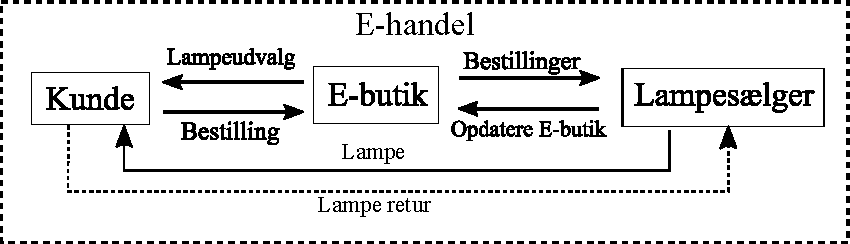
\includegraphics{e_handel_med_lampe}
	\caption{Princippet bag handel af en lampe via en e-butik.}
    \label{fig:e_handel_med_lamper}
\end{figure}

På figur \ref{fig:e_handel_med_lamper} er det vist, hvordan e-handlen starter med, at kunden får et udvalg af lamper fra e-butikken. Kunden sender så en bestilling, som via e-butikken sendes videre til lampelampebutikker, og til sidst sendes lampen til kunden. Dog ender handlen ikke nødvendigvis her, da kunden kan sende lampen retur såfremt at de gældende lovgivninger og købsbetingelser muliggør dette. For at undersøge lovgivningen nærmere kan man tage udgangspunkt i den danske lov om forbrugeraftaler\cite{retsinformationen}.

%
Lov om forbrugeraftaler

LOV nr 1457 af 17/12/2013 Gældende
(Forbrugeraftaleloven)
Offentliggørelsesdato: 18-12-2013
Justitsministeriet
%

I lovens kapitel 1, § 1, stk. 2, nr. 1 fremgår det, at lovens bestemmelser for fortrydelsesret gælder for aftaler, som er indgået ved fjernsalg. For en  fjernsalgsaftale gælder der, at aftalen om varer, er indgået gennem fjernkommunikation, hvor den erhvervsdrivende og forbrugeren ikke mødes fysisk (jf. kap. 1, § 3, nr. 1).

Ser man nu på loven i forbindelse med e-handel, foregår fjernkommunikationen gennem internettet via e-butikken, hvor fjernsalgsaftalen udføres i form af brugerens bestilling af f.eks. en lampe. Dette gør at fortrydelsesretten gælder ved e-handel.

Fortrydelsesretten er en forbrugers mulighed for at melde sig ud af en aftale, herunder køb af lamper ved e-handel. Hvis en forbruger eksempelvis køber en lampe via en e-butik, har forbrugeren mulighed for at fortryde købet inden 14 dage ved at meddele dette til den erhvervsdrivende (jf. kap. 4, § 19). Herefter har forbrugeren 14 dage til at returnere varen (jf. kap. 4, § 24). Hvis varens værdi er forringet som følge af forbrugerens unødvendige håndtering af varen for at inspicere denne, så hæfter forbrugeren for værdiforringelsen (jf. kap. 4, § 24, stk. 5). Dvs. at hvis en bruger installerer og bruger lampen, hvor der f.eks. tilpasses ledninger, så kan lampens værdi forringes og forbrugeren skal hæfte for dette. 

\subsubsection{Sammenligning af detail- og e-handel}
Ud fra ovenstående redegørelse af de to typer for handel, analyseres disse nu med henblik på at finde ligheder og forskelle, hvoraf det kan afgøres i hvilken af de to typer af handel, at problemet er størst. 

Da det initierende problem er, at forbrugeren ikke kan visualisere lampen uden at købe den, er det derfor relevant, at se på i hvor høj grad dette er tilfældet ved de to typer handler.

Fordelen ved detail-handel er, at forbrugeren ofte kan se lampen i butikken, og ud fra dette, vurdere hvilken lampe der opfylder de behov som forbrugeren har. Dog er problemet stadig, at forbrugeren ikke ser lampen i den rette kontekst, dvs. i sit eget hjem. Dette kan gøre, at forbrugeren får et godt indtryk af lampen i den kontekst, som butikken præsenterer den i, men at den ikke passer ind i den kontekst, som forbrugeren køber lampen til.

Ved e-handel har forbrugeren ikke muligheden for, at se en fysisk udgave af lampen, men ofte kun billeder. Dette gør at forbrugeren alene kan tage valg ud fra de billeder og informationer som e-butikken præsenterer. Problemet er så, at billederne til dels ikke er interaktive, dvs. brugeren ikke kan se lampen fra flere vinkler end dem som billederne er taget i, samt at billederne ikke er taget af lampen i den kontekst, som forbrugeren ønsker at købe lampen til. 

Med hensyn til konteksten er fordelen ved e-handel, at forbrugeren kan sidde derhjemme, i den kontekst, hvor lampen skal indgå, og sammenligne med de informationer, der er tilgængelige på e-butikken. I modsætning til dette er detail-butikker, hvor forbrugeren står i butikken, og måske har problemer med at huske eller blot forestille sig alle detaljerne ved den kontekst, som lampen skal indgå i.

Ud fra denne sammenligning, er der på den ene side detail-handel, hvor det er svært at visualisere konteksten, men hvor man kan se lampen. På den anden side er e-handel, hvor man kan sidde derhjemme i konteksten, men har svært ved at visualisere lampen. 

For at afgøre hvilken type handel denne rapport vil fokusere på, skal der derfor svares på om det er mangel på visualisering af lampen i kontekst ved detail-handel eller mangel på visualisering af lampen ved e-handel, som er det største problem.

Da forbrugeren omgås og ser den kontekst, som lampen skal indgå i f.eks. et kontor, køkken og bad, så må man kunne antage at forbrugeren har en forestilling om, hvordan denne kontekst ser ud selvom forbrugeren ikke står i den når der handles i en fysisk butik. Derfor er dette ikke et lige så stort problem, som hvis forbrugeren ikke kan visualisere lampen når der handles via e-handel. Derfor vil fokuset i denne rapport være at forbedre forbrugerens evne til at visualisere lamper under e-handel.

\subsubsection*{Opsummering}
Trods at problemet opstår hos forbrugeren altså, at de har problemer med at visualisere den givne lampe fra alle vinkler og i det rette miljø, er der ingen måde, hvorpå forbrugeren selv kan løse dette problem på en let og effektiv måde. Vi vil derfor fokusere på hvordan problemet kan blive løst allerede før varen når ud til forbrugeren. Derfor er vi nødt til at fokusere på lampebutikker (e-handelsbutikker), når det kommer til løsningen af visualiserings-problemet. Her kunne det tænkes, at der kunne udarbejdes et værktøj, der ville forbedre og optimere forbrugerens visualisering af den givne lampe.
